\documentclass[11pt]{article}
\usepackage[utf8]{inputenc}
\usepackage[english]{babel}
\usepackage{amsmath}
\usepackage{dsfont}
\usepackage{graphicx}
\usepackage{float}
\usepackage{lipsum}
\usepackage{multicol}
\usepackage{xcolor}
\usepackage{tabularx}
\usepackage{booktabs}
\usepackage{hyperref}
\usepackage{wrapfig}
\usepackage{listings}

\newcolumntype{Y}{>{\centering\arraybackslash}X}
\usepackage[left=2.00cm, right=2.00cm, top=2.00cm, bottom=2.00cm]{geometry}

\title{AN2DL Reports Template}

\begin{document}
    
    \begin{figure}[H]
        \raggedright
        
\includegraphics[scale=0.4]{figures/polimi.png} \hfill 
\includegraphics[scale=0.3]{figures/airlab.jpeg}
    \end{figure}
    
    \vspace{5mm}
    
    \begin{center}
        % Select between First and Second
        {\Large \textbf{AN2DL - First Homework Report}}\\
        \vspace{2mm}
        % Change with your Team Name
        {\Large \textbf{DeepL}}\\
        \vspace{2mm}
        % Team Members Information
        {\large Matteo Bonfadini,}
        {\large Elena Lippolis,}
        {\large Lorenzo Cossiga,}
        {\large Michele Baggi}\\
        \vspace{2mm}
        % Codabench Nicknames
        {50mgk,}
        {elenali,}
        {lorenzocossiga,}
        {mik01}\\
        \vspace{2mm}
        % Matriculation Numbers
        {243786,}
        {252310,}
        {242309,}
        {252119}\\
        \vspace{5mm}
        \today
    \end{center}    
    \vspace{5mm}
    
    \begin{multicols*}{2}        
        \section{Introduction}

        The project aims to implement \textit{multi-class image classification} using \textbf{deep learning} techniques for blood cell analysis. This \textit{supervised learning} task requires balancing model complexity to ensure generalization to unseen data while minimizing \textit{overfitting}. The primary \textbf{goal} is to design a solid neural network that classifies blood cells into the correct categories with high accuracy.
        
        The \textbf{approach} involves dataset analysis to identify potential issues such as class imbalance, image quality, and the need for preprocessing. We then developed simple deep learning models to establish a performance benchmark, which was subsequently refined into more complex models.
        
        \section{Problem Analysis}

        The dataset consists of \textbf{13759} RGB images designed for the classification of different types of blood cells. Each image has size 96x96 pixels and it is labeled with one of eight (from 0 to 7) classes, representing the following blood cell types: basophils (0), eosinophils (1), erythroblasts (2), immature granulocytes (3), lymphocytes (4), monocytes (5), neutrophils (6), and platelets (7). We show in Figure~\ref{fig:dataset} a sample for each class.

        \begin{figure}[H]
            \centering
            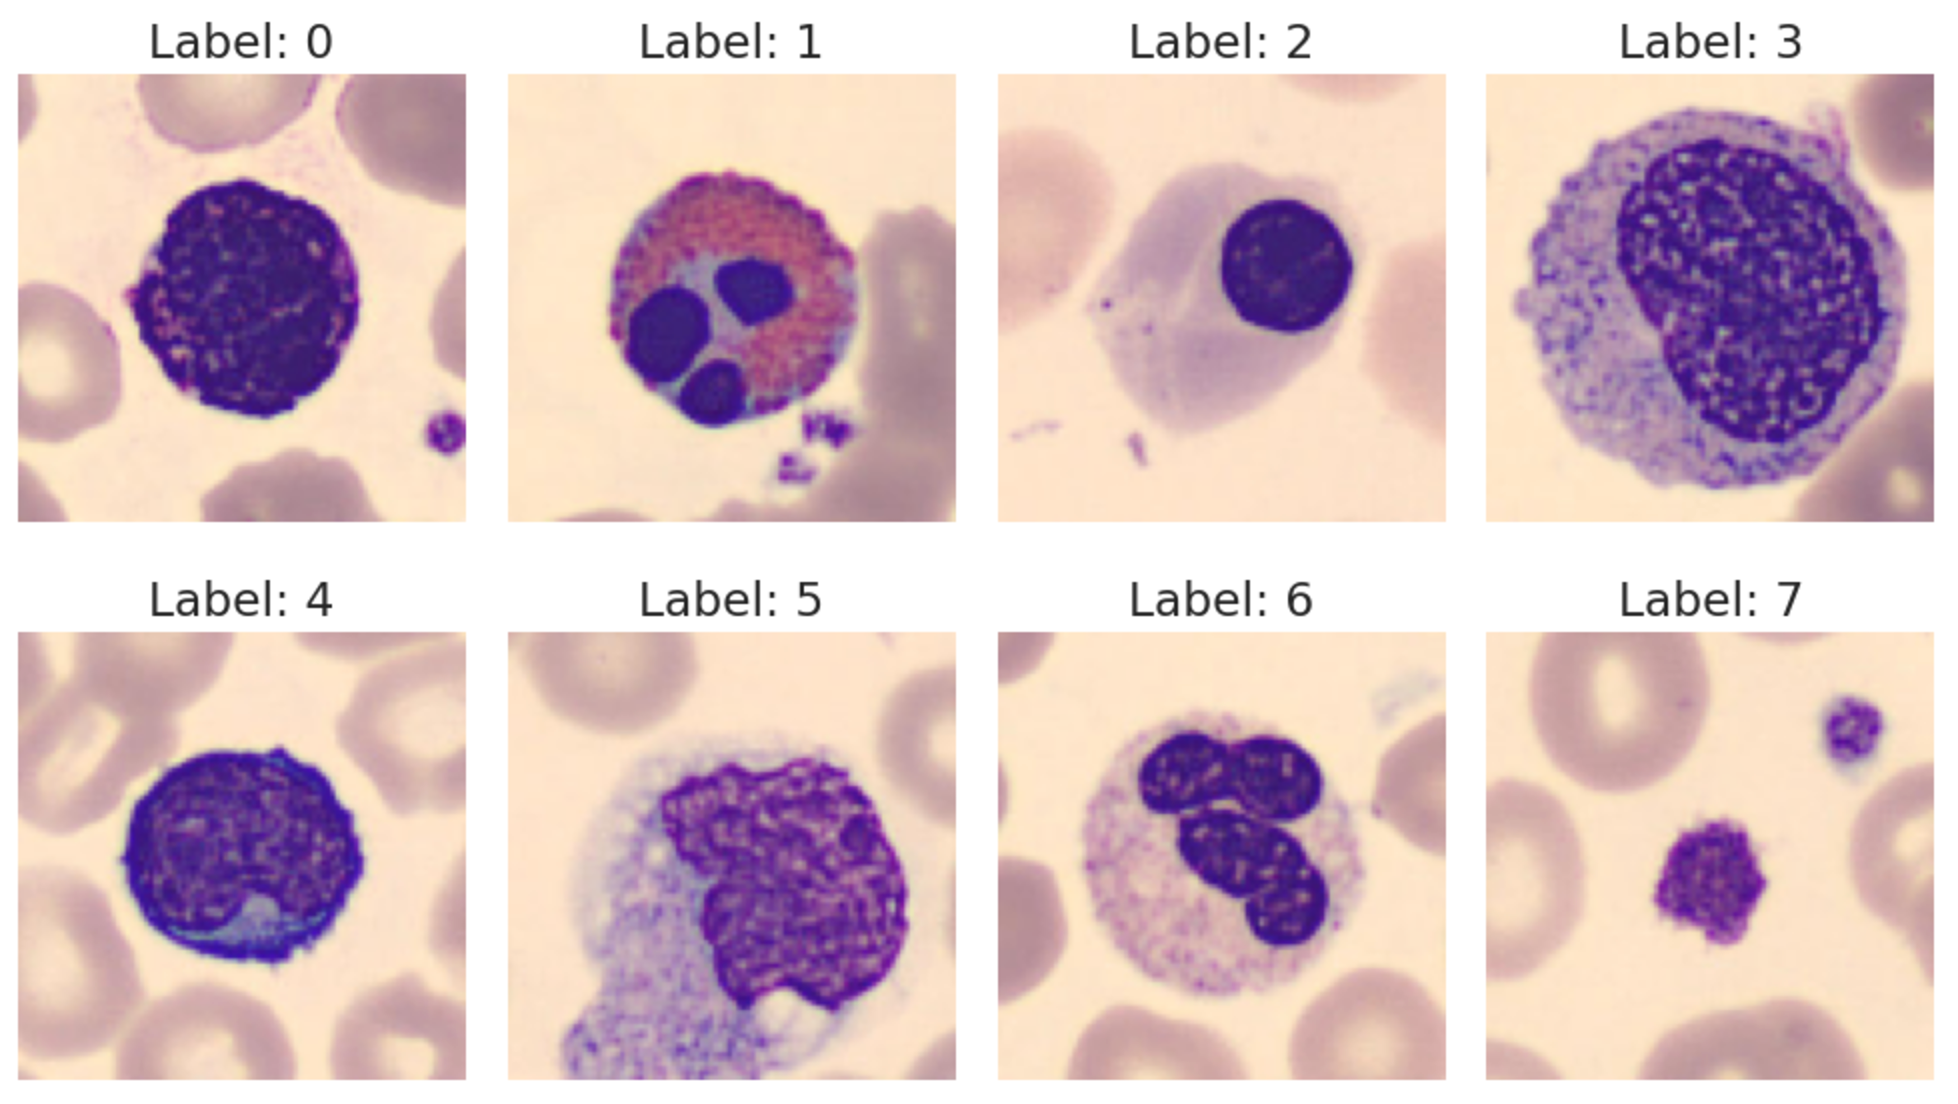
\includegraphics[width=\linewidth]{figures/SCR-20241122-nvwz.png}
            \caption{Example of an image for each class}
            \label{fig:dataset}
        \end{figure}

        We tackled the problem in a 3-phase approach.

        \subsection{Phase 1: Data Inspection}

        Firstly, we inspected the dataset and printed its shape. Secondly, a deeper inspection revealed the presence of \textit{obvious} outliers, as shown in Figure~\ref{fig:rickroll}, which could skew the learning process: 200 samples of the very same blood cell for each class and 200 rick roll. Therefore we proceed by erasing those images.

        We also noticed some images with grayscale backgrounds, but further analysis through \textit{PCA} based on the Mahalanobis distance \cite{outliers} (normalizing the dataset) showed this pattern did not negatively influence our performance. This indicates that the grayscale background images do not impact the model's ability to learn effectively. 

        % \begin{table}[H]
        %     \centering
        %     \setlength{\tabcolsep}{1pt}
        %     \caption{Shape of the dataset.}
        %     \begin{tabularx}{\linewidth}{lYY}
        %         \toprule
        %         & Class & Number of samples \\
        %         \midrule
        %         & 0 & 1052  \\
        %         & 1 & 2381  \\
        %         & 2 & 1285  \\
        %         & 3 & 2226  \\
        %         & 4 & 1049  \\
        %         & 5 & 1393  \\
        %         & 6 & 2530  \\
        %         & 7 & 1843  \\
        %         \midrule
        %         Total: & \textbf{8}  & \textbf{13759} \\
        %         \bottomrule
        %     \end{tabularx}
        %     \label{tb:class-shape}
        % \end{table}

        \begin{figure}[H]
            \centering
            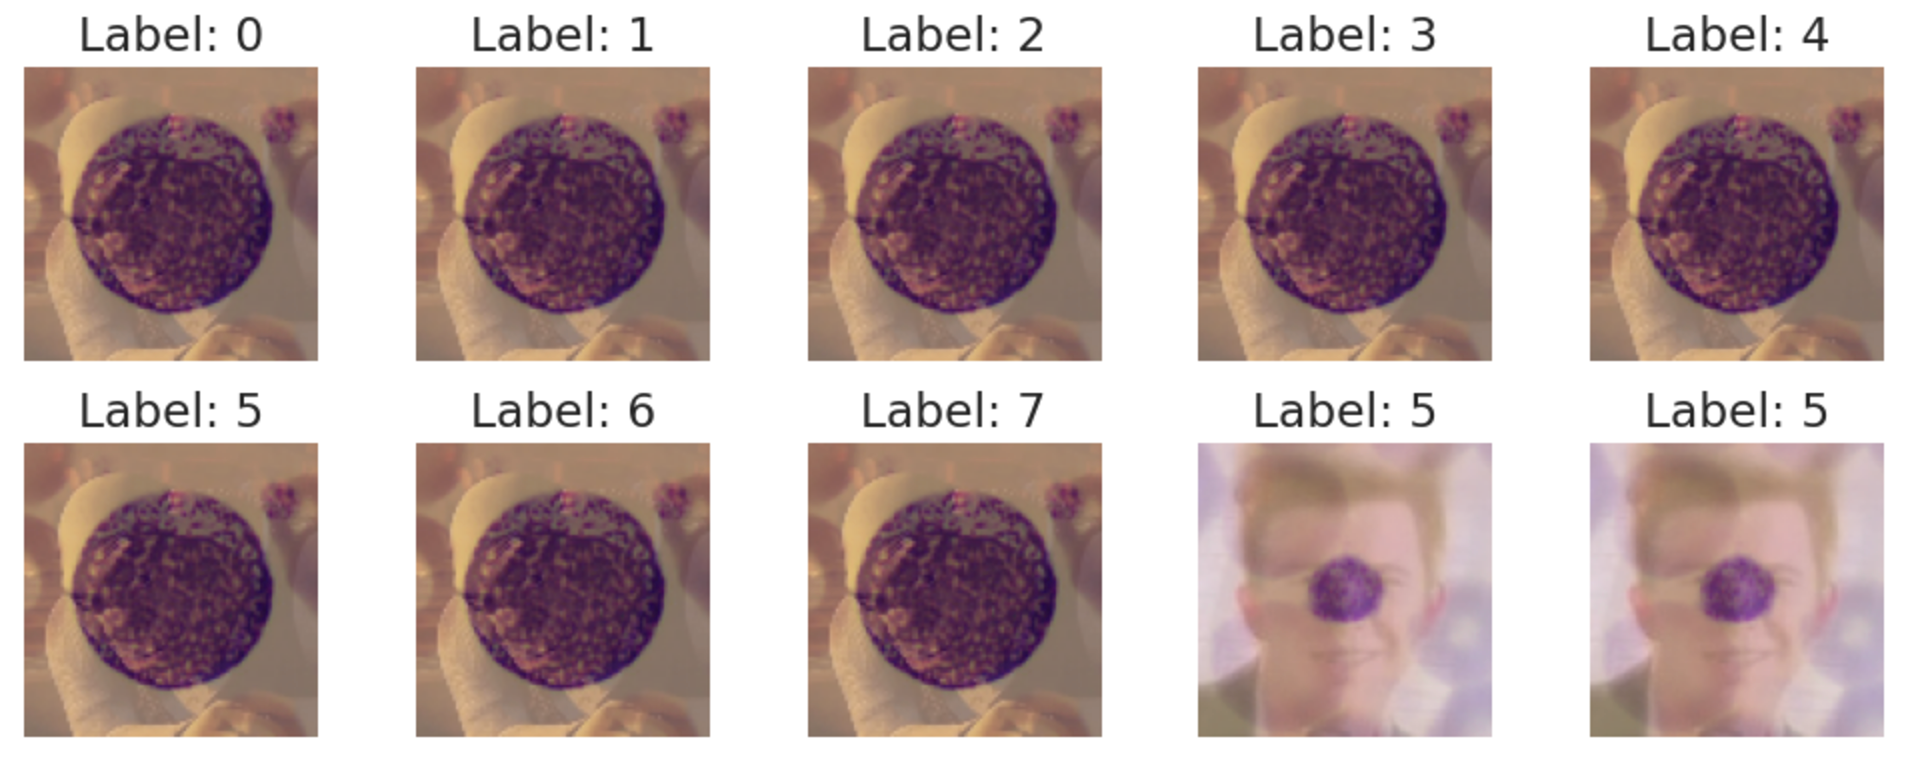
\includegraphics[width=\linewidth]{figures/SCR-20241122-oigg.png}
            \caption{Samples of \textit{obvious} outliers.}
            \label{fig:rickroll}
        \end{figure}

        \subsection{Phase 2: Class Imbalance}

        The new dataset, for a total of \textbf{11959} blood cell images, has shape reported in Figure~\ref{fig:imbalance}.

        \begin{figure}[H]
            \centering
            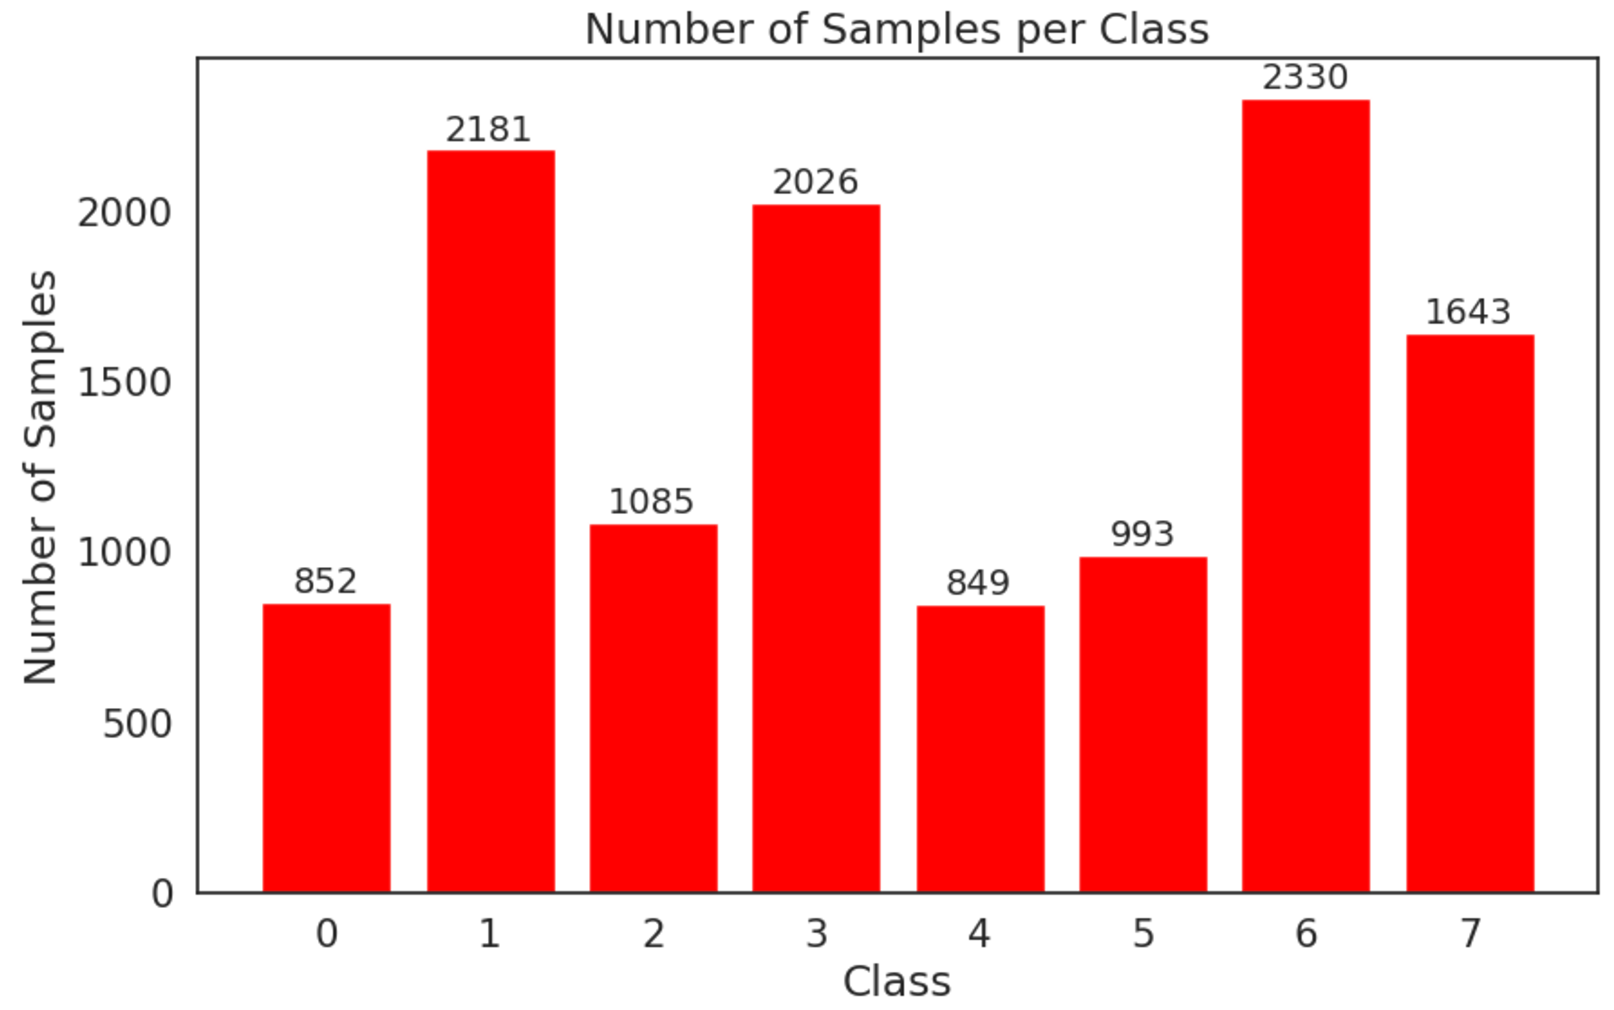
\includegraphics[width=0.75\linewidth]{figures/SCR-20241122-ooty.png}
            \caption{Number of samples in each class.}
            \label{fig:imbalance}
        \end{figure} 

        \noindent Upon closer inspection, one might observe that the dataset exhibits class imbalance. This problem poses additional challenges for training a model that generalizes effectively across all categories.

        To address this, after the splitting of the dataset into training, validation and test sets according to an 83:13:4 ratio, we balanced the training one by replicating images in the underrepresented classes. The result is a new training set with 2000 images for each class.

        Throughout the challenge we noticed that the validation accuracy and the (local) test accuracy were almost identical, as a matter of fact in some training session we just split the data 83:17, therefore we are not going to show the test accuracy for the various models as it would be redundant with respect to the validation one.

        Finally, we applied \textbf{data augmentation techniques} to create variations of these images (\textit{oversampling}) \cite{oversampling}. In particular, after trials and errors, we decided to use \texttt{AugMix} and \texttt{RandAugment} \cite{aug}.

        

        \subsection{Phase 3: Mixed Precision}

        One of the main challenges we encountered was the low training speed, which was solved by implementing mixed precision \cite{mixed-precision}. This technique uses lower precision (16-bit floating point numbers) for computations while retaining single precision (32-bit) for weight updates. Mixed precision accelerated training and reduced energy consumption, all while maintaining a reasonable accuracy level. 

        \subsection{Overfitting and Assumptions}
        
        Overfitting of the training set reduced the model's ability to perform well on unseen (and possibly \textit{modified}) test data. We intentionally allowed initial overfitting assuming that we needed to verify that the model was able to fit the training data before addressing generalization issues, to employ only later techniques like early stopping and dropout layers to mitigate overfitting and enhance performance on unseen data \cite{overfitting}.

        Finally, we assumed the dataset to be solid, with minimal labeling error or inconsistencies. Moreover, we hypothesized that a simple baseline model would provide reasonable performance before moving to more complex architectures. 

        % The last assumption we made was that Codabench would not let us down when we needed it to test our final models ... apparently that was a bit too much to ask for.

        %\begin{figure}[H]
            %\centering
            %\includegraphics[width=0.3\linewidth]%{meme/pablo.png}
        %\end{figure}

        \section{Method}
        
        To tackle the classification task, we employed a \textbf{transfer learning} approach, leveraging pre-trained models as feature extractors. Specifically, we experimented with three different architectures: VGG16, EfficientNetV2B0, and an additional model structurally identical to VGG16.
        
        For the VGG16-based model, the architecture consisted of a dense layer with linear transformation, batch normalization to stabilize and accelerate training, ReLU activation to introduce non-linearity, a dropout layer (dropout rate = 0.3) for regularization, and a final dense layer with softmax activation for multi-class classification:

        \begin{center}
        \begin{tabular}{c}
        \toprule
        vgg16\\
        \hline
        Dense(256)\\
        Batch Normalization\\
        Dropout\\
        Dense(8)\\
        \bottomrule
        \end{tabular}
        \end{center}

        For EfficientNetV2B0, we used a more complex setup to improve generalization and robustness:

        \begin{center}
        \begin{tabular}{c}
        \toprule
        effNetV2B0\\
        \hline
        Augmentation\\
        Dense(256)\\
        Batch Normalization\\
        Dropout\\
        Dense(256)\\
        Batch Normalization\\
        Dropout\\
        Dense(8)\\
        \bottomrule
        \end{tabular}
        \end{center}
        
        The models were built using the Keras Functional API, linking the input layer to the custom head via the frozen vgg16/effNet feature extractor. The model were later compiled with a loss function (Categorical Cross-Entropy, designed for multi-class classification tasks), and the \textbf{Lion optimizer} \cite{lion}. Furthermore, during the training phase, we exploited the callbacks \textbf{early stopping}, \textbf{reduce learning rate} and \textbf{module checkpoint} to prevent overfitting and adjust the learning rate.

        \section{Experiments and Results}
        
        Initially, we implemented a simple model based on the CIFAR-10 architecture. While it achieved acceptable performance on the validation set, its accuracy on the hidden test set was suboptimal.
        
        To address this, we developed a more complex model identical to VGG16 but trained from scratch with randomly initialized weights. Although this approach slightly improved test accuracy, the gains were limited.
        
        Subsequently, we shifted to transfer learning, incorporating pre-trained models (VGG16 and EfficientNetV2B0). For VGG16, we added a custom classification head as described earlier and fine-tuned the model. This approach achieved the best test set accuracy of 82\%.
        
        We also experimented with EfficientNetV2B0 with additional dense and augmentation layers.
        
        The results on both validation and hidden test set are shown in Table~\ref{tb:Measurements}. These results emphasize that simplicity, combined with fine-tuning of higher convolutional layers in pre-trained models, can yield better results in our scenario.
    
        \begin{table}[H]
            \centering
            \setlength{\tabcolsep}{3pt}
            \caption{Various models accuracy.}
            \begin{tabularx}{\linewidth}{lYY}
                \toprule
                Model & Val. Acc. & Hidden Test Acc. \\
                \midrule
                Cifar10 & 83.24\% & 25\% \\
                vgg16$_{RI}$ & 82.59\% & 39\%\\
                vgg16$_{TL}$ & 74.63\% & 49\% \\
                \textbf{vgg16$_{FT}$} & \textbf{97.13\%} & \textbf{82\%} \\
                effnet$_{FT}$ & 96.20\% & 75\% \\
                \bottomrule
            \end{tabularx}
            \label{tb:Measurements}
        \end{table}

        \section{Conclusions}

        This project aimed to solve a multi-class classification problem with a dataset of blood cell images using transfer learning and fine-tuning with VGG16. The algorithm includes augmentation, regularization, and training techniques, achieving high accuracy in both validation and test datasets, and demonstrating its potential applicability in medical image analysis.

        
        The final VGG16 model achieved high performance on validation and test accuracy, demonstrating the effectiveness of transfer learning and fine-tuning. Leveraging the pre-trained VGG16 model allowed a more effective extraction and use of complex visual features, reducing the need for training from scratch and speeding up convergence. Augmentation and regularization techniques helped mitigate overfitting and improve generalization across all blood cell classes, and the use of mixed precision reduced computational overhead and accelerated training. 
        
        Several areas for improvement in our models include addressing some \textbf{weaknesses}, such as the drop in accuracy from validation to test data, indicating the model could still struggle with generalizing to unseen data. In addition, given the dataset's initial class imbalance, it is possible that certain underrepresented blood cell types experienced lower performance metrics. A further improvement in our algorithm could be adjusting the loss function to prioritize minimizing critical misclassification and using more sophisticated methods for dealing with class imbalance.

        To conclude, even though we did most of work together, we highlight here the main contribution of each team member: Lorenzo and Michele developed the VGG16 and EfficentNet models, while Elena and Matteo dealt with data inspection and augmentation as well as the writing of this report.

        \bibliography{references}
        
        \bibliographystyle{abbrv}
    
    \end{multicols*}







\end{document}